% Chapte 9
\chapter{Advertisement enhancement} % Main chapter title

\label{Chapter9} % For referencing the chapter elsewhere, use \ref{Chapter1} 
\newpage






\section{Introduction}




Advertisement enhancement is another follow-up study of the previous experiment in which the body interaction was found to be the most attractive and engaging advertisement compared to the other two techniques (Non-interactive and mobile Interactive), 






\section{Advertisement enhanced version}

The advertisement interface was exactly the same, but the only change was brought in it was the integration of multiple Kinect cameras to cover the sides of the screen, a person passing from the side could see his self at the side of the screen and when moving to the middle of the screen the camera could smoothly transition the person from side camera to the center camera by having the same silhouette color, physically the cameras are positioned side-by-side therefor there is a small gap for each camera range, which is also not perceivable by passers-by. Refere to chapter 7 for more technical details.


\begin{figure}[H]
    \centering
    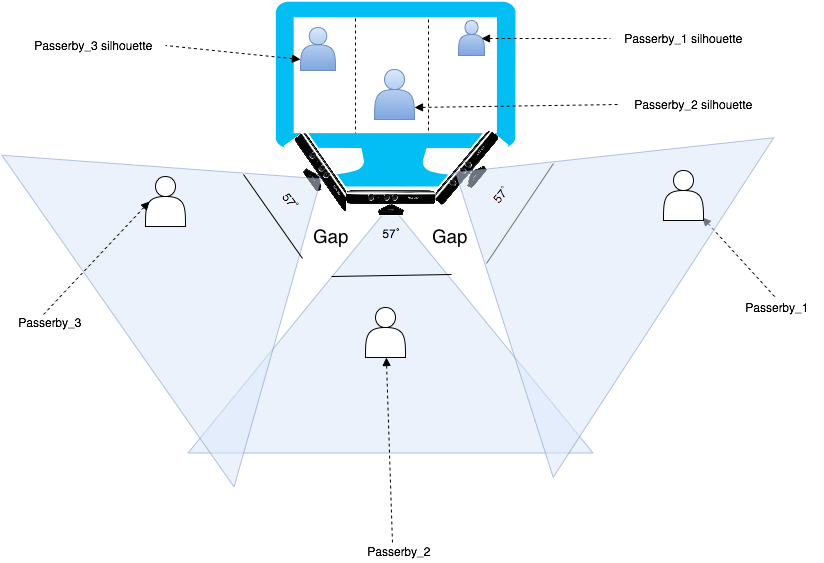
\includegraphics[width=110mm,height=70mm]{Figures/9/Kinect_Extended}
    \caption{Advertisement extended version using three Kinect cameras.}%
    \label{fig:KinectExtended}%
\end{figure}




\section{Research question}
This experiment was conducted to find out that what are the major effects when the coverage area is expanded in both right and left side of the screen.

\begin{enumerate}
\item Would the attention level change?
\item Would the number of engaged passers-by increase?
\item Would the average engagement time rise?
\item Would there be any changes in number of Honeypot and landing effect?
\item What would be other passer-by behavior to the screen?
\end{enumerate}



\section{Design study}

\subsection{Location}
The same location that the last experiment was conducted was chosen again, it was in Weimar tourist information center, It was positioned in the same pathway of passers-by. 


\subsection{Duration}
This experiment was conducted only with advertisement’s extended version for three continues days; the days were the crowded days of the week (Friday, Saturday, Sunday), 

\subsection{Participants}
The participants were from Tourist information center; they were not informed that there is an interactive screen. Most of the participants were of old age, and the rest were middle aged and young aged participants. 

\subsection{Data gathering}
The bellow types of data were gathered during three days.


\begin{enumerate}
\item \textbf{On-Site Observation} \\
Observation periods were selected the same as the previous study, from 10:00 – 12:00 and the second was from 14:00 – 16:00, During these two time slots the bellow observations were made.

\begin{enumerate}
\item \textbf{Attention Level measurement} \\
Number of glances and number of ignores were counted by observing the passers-by from a fixed location, anyone who turned his/her face less than 3 seconds were counted as glance, see the full report of glances in Appendix \ref{AppendixE}.1

\item \textbf{Passerby behavior} \\
The behaviors of the passers-by were observed by direct observation in onsite and also from the Camera depth recorded frames. From the observation two important effects were taken in consideration (honeypot and landing effect).


\end{enumerate}

\item \textbf{Colored-image recording} \\
A 2D colored image was taken per second from each of three cameras, and meanwhile were joint together side-by-side and after the image recording was done, in lab another post processing script was applied to integrate a static background using Adobe Photoshop application. To match the data logs and the image frames each image name consisted time as (12.43.21.png).
Bellow three kinect images stacked together, as can be seen that people' colored images rendered on the images (1,2 and 3) these images are stacked together so that the transition of one person be smooth from one camera to the other.

\begin{figure}[H]
   \centering
    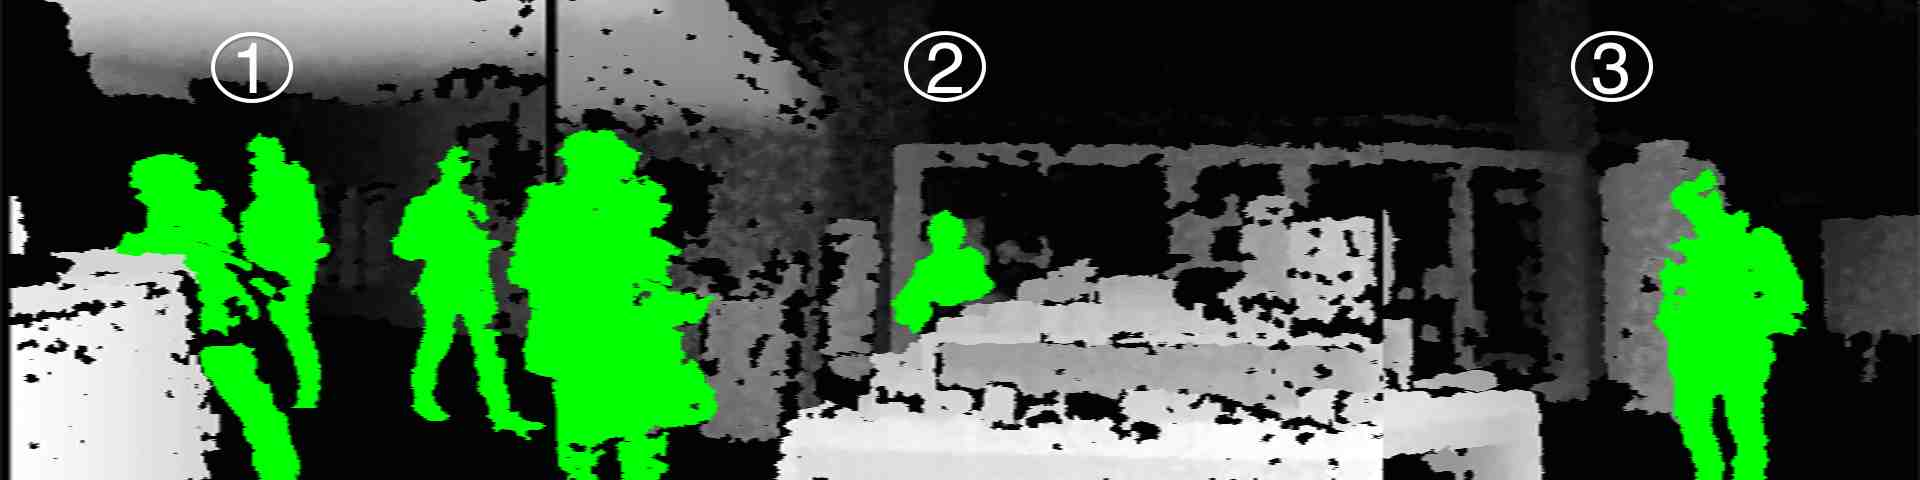
\includegraphics[width=\textwidth,height=40mm]{Figures/9/stacked_image}%
    \caption{Three Kinect images}%
    \label{fig:threekinectimages}%
\end{figure}

\end{enumerate}


\newpage
\section{Findings and results}

\subsection{Attention Level measurements}

The bellow chart shows the number of glances and ignore for the following three days.
\begin{figure}[H]
    \centering
    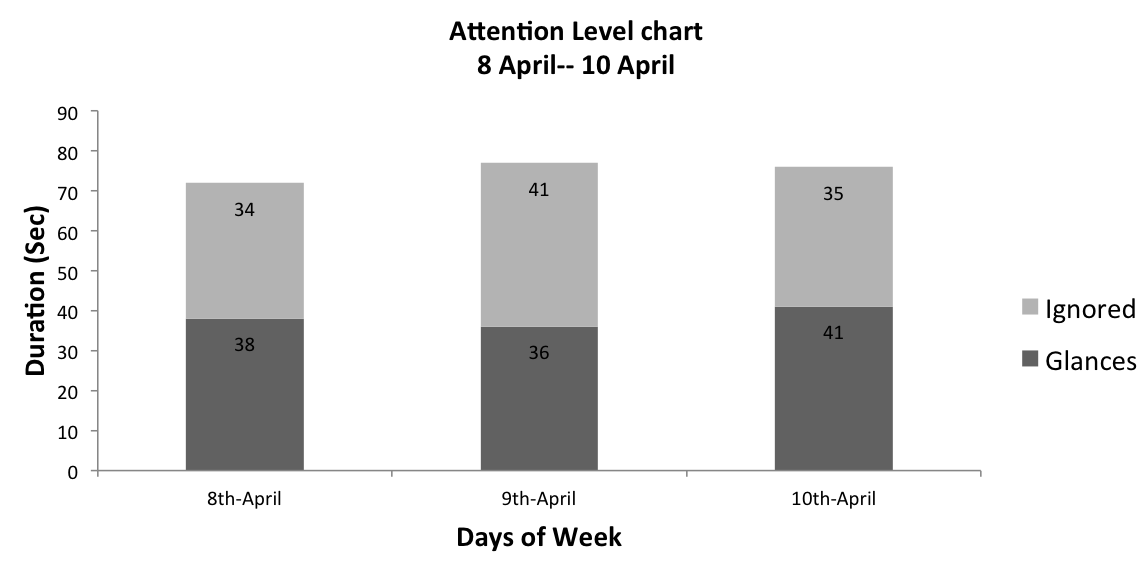
\includegraphics[width=110mm,height=55mm]{Figures/9/newbody_Inter_chart}%
    \caption{Attention level chart}%
    \label{fig:newbodyattentionlevelchart}%
\end{figure}


As can be seen from the above chart every day has almost similar number of glances and ignores and in average it makes about \%51 glances and \%49 ignores which is a great difference compared to the previous body interactive advertisement.


\begin{figure}[H]
    \centering
    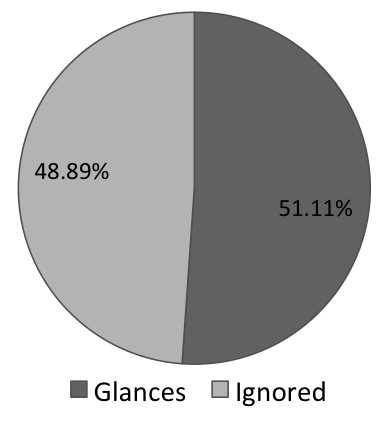
\includegraphics[width=70mm,height=55mm]{Figures/9/newbody_inter_percentage}
    \caption{Attention level percentage}%
    \label{fig:Nonattentionlevelpercentage}%
\end{figure}



\subsection{Engagement phases and duration spent}

The engagement time for phases were measured from system logs and depth recording manually and in which people spent 16.10 seconds in average for the motivation phase some people took longer and some shorter, and some of them may have left without switching to the rest phases. 16.20 seconds in average was spent for interaction phase, which was different from person to person, and only 3.63 seconds in average was spent for video advertisement.

\begin{figure}[H]
    \centering
    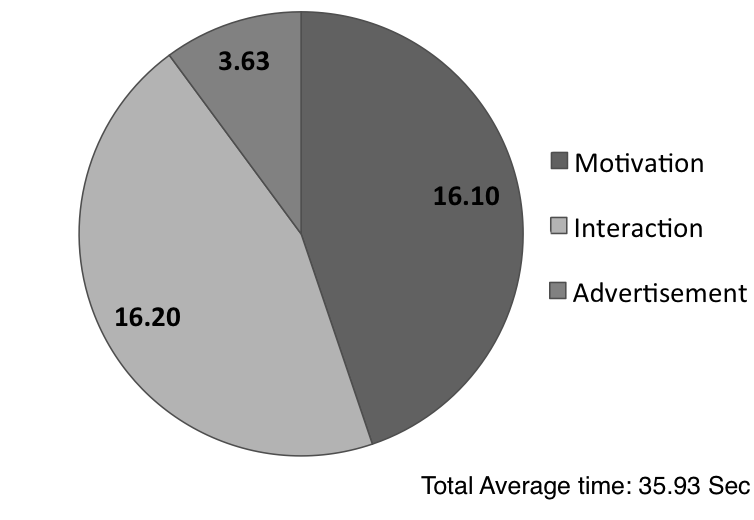
\includegraphics[width=90mm,height=60mm]{Figures/9/avg_phases}
    \caption{Average time for each phase}%
    \label{fig:newbodyaveragephases}%
\end{figure}



\subsection{Passerby and engagement}

The entire number of passers-by and engaged people were counted manually and people who interacted for more than 3 seconds were flagged as engaged. As shown in the chart bellow all three days are individually recorded. 

\begin{figure}[H]
    \centering
    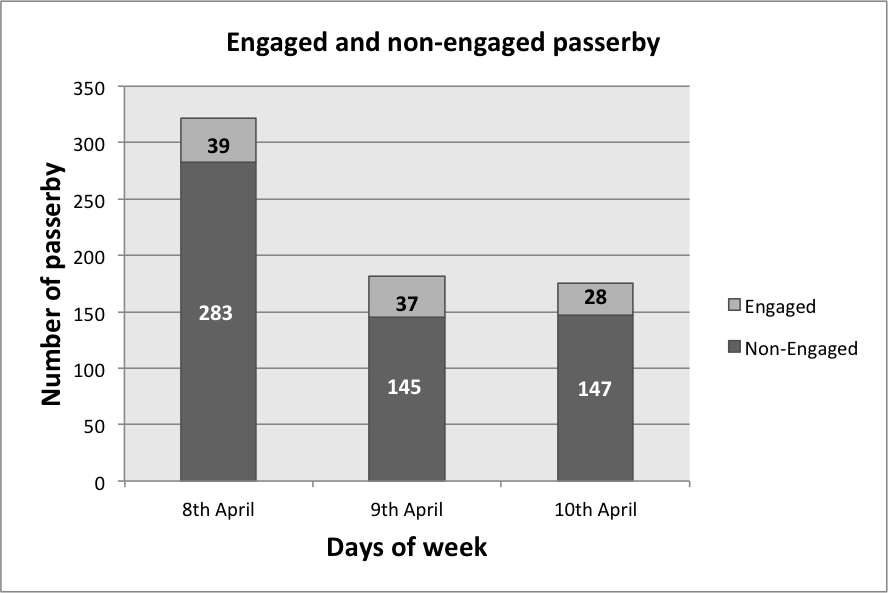
\includegraphics[width=110mm,height=60mm]{Figures/9/newbody_inter_engage_day}
    \caption{New body interaction Number of engaged passerby}%
    \label{fig:newbodyengagedandengagedby}%
\end{figure}


From entire passers-by \%15.32 of them were engaged with the display and the rest might have only glanced or simply ignored.

\begin{figure}[H]
    \centering
    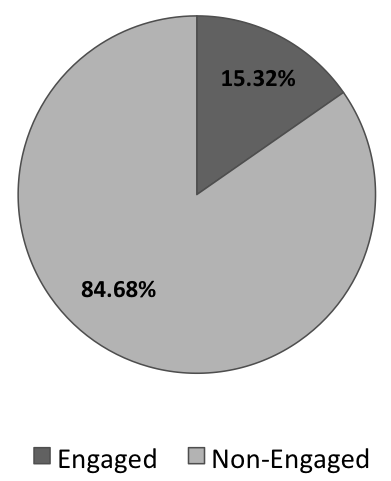
\includegraphics[width=70mm,height=60mm]{Figures/9/newbody_eng_percentage}
    \caption{Percentage of engaged and passers-by}%
    \label{fig:newbodyengagedpasserbypercentage}%
\end{figure}


\subsection{Landing and Honeypot effects}

Landing and honeypot effects were observed for this type of technique although the number of days was only for three days. 


\begin{figure}[H]
    \centering
    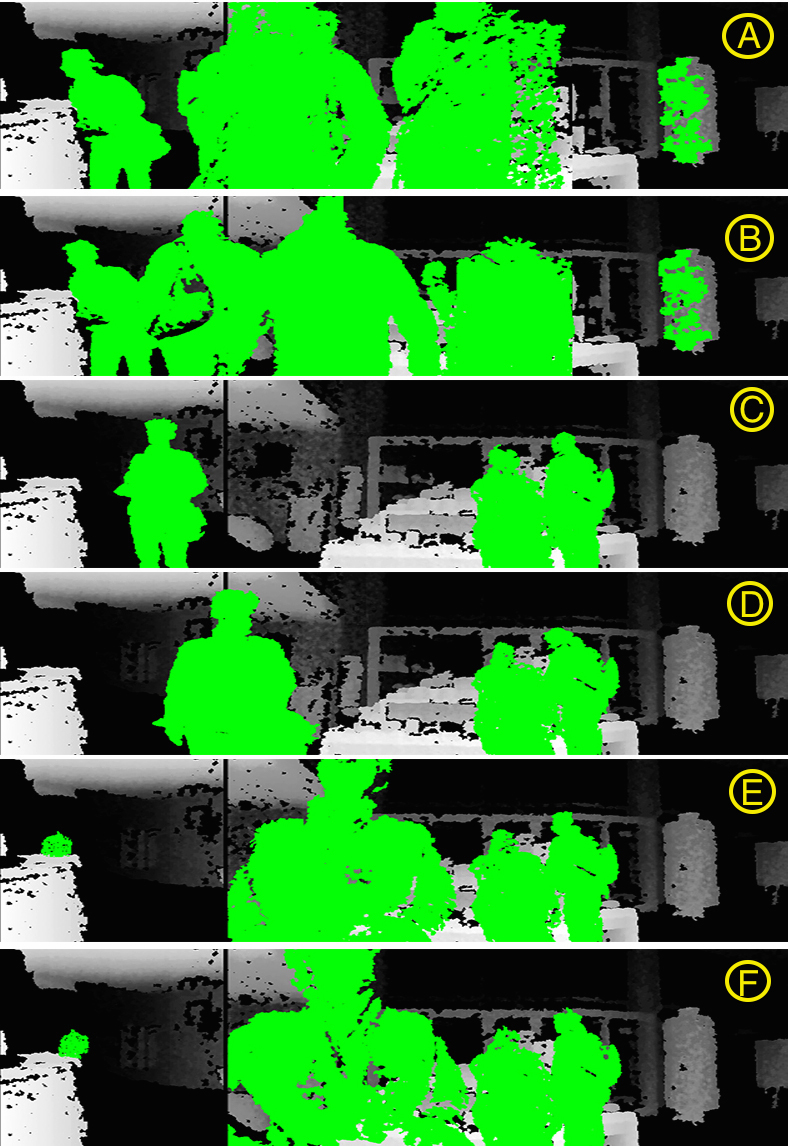
\includegraphics[width=\textwidth,height=140mm]{Figures/9/effects/honeypot}
    \caption{Honeypot effect}%
    \label{fig:newbodyhoneypoteffect}%
\end{figure}

As can be seen from the picture above, in first frame (A) two person in the middle are engaged with the system and a women at the right is busy with the help desk, but she is attracted to the screen and has looked many times in previous frames, in (B) the two guys leave and in Frame (C) that women is left alone and then approaches toward the screen in frame (D and E) and starts actively interaction in frame (F).

Few landing effects has also been happened which were similar like previous some noticed the interactivity in the middle and stopped and moved back toward the screen.  

The chart bellow shows the frequencies of landing and honeypot effects.

\begin{table}[H]
\caption{Landing and honeypot effects}
\label{tab:landingandhonypot}
\centering
\resizebox{8cm}{0.8cm}{ 
\begin{tabular}{| l | c | c |}
\toprule
\tabhead{Days} & \tabhead{Landing effect} & \tabhead{Honeypot effect} \\
\midrule
8th April & 3 &  3 \\
9th April  & 2 &  5 \\
10th April  & 1 &  2 \\
\bottomrule
\end{tabular}
}
\end{table}







\subsection{Other observations}
see Appendix Appendix \ref{AppendixE}.2





\newpage
\subsection{Comparison with Body interaction}


\begin{enumerate}


\item \textbf{Comparison of number of passers-by} \\
To be on safe side that the number of participants were statistically the same the bellow computation has be applied on three similar days, which provides the base for further evaluations.

\begin{table}[H]
\caption{Number of people for three conditions}
\label{tab:newbodypasserbyofthreeweeks}
\centering
\resizebox{8cm}{1cm}{  
\begin{tabular}{| l | c | c | c |}
\toprule
\tabhead{Days} & \tabhead{Non-Interactive} & \tabhead{Body Interactive} & \tabhead{Enhanced body Interactive} \\
\midrule
\textbf{Day 1}  & 212 & 259 &  322 \\
\midrule
\textbf{Day 2}  & 209 & 216 &  182 \\
\midrule
\textbf{Day 3}  & 208 & 122 &  175 \\
\midrule
\textbf{Total}  & 629 & 597 &  679 \\
\bottomrule
\end{tabular}
}
\end{table}
ANOVA test revealed that there is no statistical significant different between the passers-by in each of the conditions (\emph{(F2,3)=0.1449, p >.05 (p=0.868)})



\item \textbf{Attention Level comparison}  \\
The number of glances and ignores for both body interaction and enhanced body interaction was collected as bellow.


\begin{table}[H]
\caption{Cross tabulation for each condition attention level}
\label{tab:newbodycrosstabulationweeks}
\centering
\resizebox{8cm}{1cm}{ 
\begin{tabular}{| l | c | c | c |}
\toprule
\tabhead{Method} & \tabhead{Glanced (\%)} & \tabhead{Ignored} & \tabhead{Total } \\
\midrule
\textbf{Body Interactive}     	 & 106 (\%41.40)   &   150      &   256\\
\midrule
\textbf{New body Interactive }   & 115 (\%51.11)  &   110      &   225\\
\midrule
\textbf{Total }         		 & 221            &   260      &   481\\
\bottomrule
\end{tabular}
}
\end{table}

As can be seen the new body interactive advertisement has a higher percentage about \%51 of the glances compared to the old body interactive advertisement, this means that a rise of \%10 the number of glances have been increased. To examine if these have statistically significant difference, the Chi-square test was applied on them and revealed ${\chi}^2$\emph{(1, N=481)=4.5413, p < .05 (p=.033086)} that they are statistically different and the new body attraction technique does have higher effect the attention level.


\item \textbf{Landing effect comparison}\\
The landing effects were recorded for non-interactive, body interactive and enhanced body interactive in bellow table.

\begin{table}[H]
\caption{Cross tabulation for each condition Landing effect }
\label{tab:newbodylandingeffect}
\centering
\resizebox{8cm}{1cm}{  
\begin{tabular}{| l | c | c | c |}
\toprule
\tabhead{Method} & \tabhead{Non-Interactive} & \tabhead{Body Interactive} & \tabhead{Enhanced body Interactive } \\
\midrule
\textbf{Day 1}    & 2    &   2      &   1\\
\midrule
\textbf{Day 2 }   & 0    &   2      &   2\\
\midrule
\textbf{Day 3}    & 1    &   3      &   3\\
\bottomrule
\end{tabular}
}
\end{table}
After conducting ANOVA test, it states that there is no significant different between three days for all of the conditions.\\
(\emph{(F2,3)=1.857, p >.05 (p=0.236)})


\item \textbf{Honeypot effect comparison}\\
Honeypot effects were also gathered from those days as bellow in table.

\begin{table}[H]
\caption{Cross tabulation for each condition Honeypot effect }
\label{tab:newbodyhoneypoteffect}
\centering
\resizebox{8cm}{1cm}{  
\begin{tabular}{| l | c | c | c |}
\toprule
\tabhead{Days} & \tabhead{Non-Interactive} & \tabhead{Body Interactive} & \tabhead{Enhanced body Interactive } \\
\midrule
\textbf{Day 1}    & 2    &   2      &   3\\
\midrule
\textbf{Day 2 }   & 2    &   5      &   5\\
\midrule
\textbf{Day 3}    & 1    &   3      &   2\\
\bottomrule
\end{tabular}
}
\end{table}

ANOVA reveals that there is also no statistical difference between these conditions. \\
(\emph{(F2,3)=1.667, p >.05 (p=0.266)})



\item \textbf{Engaged and Non-engaged passerby}


\begin{table}[H]
\caption{Number of engaged passerby in three weeks}
\label{tab:engagedofthreeweeks}
\centering
\resizebox{8cm}{1cm}{  
\begin{tabular}{| l | c | c | c |}
\toprule
\tabhead{Days} & \tabhead{Non-Interactive} & \tabhead{Body Interactive} & \tabhead{Enhanced body Interactive } \\
\midrule
\textbf{Day 1}  & 15 & 26 &  39 \\
\midrule
\textbf{Day 2}  & 15 & 20 &  37 \\
\midrule
\textbf{Day 3}  & 15 & 23 &  28 \\
\midrule
\textbf{Total}  & 45 & 69 &  104\\
\bottomrule
\end{tabular}
}
\end{table}

ANOVA reveals that there is statistical difference between these conditions. \\
(\emph{(F2,3)=20.3154, p <.05 (p=0.0021)})

And conducing post-hoc Tukey HSD test, reveals that 

\begin{table}[H]
\caption{Post-Hoc Tukey’s HSD}
\label{tab:engage-non-posthoctukey}
\centering
\resizebox{\textwidth}{!}{  
\begin{tabular}{| l | c | c | c |}
\toprule
\tabhead{Methods} & \tabhead{Tukey HSD Q statistic} & \tabhead{Tukey HSD p-value} & \tabhead{Tukey HSD inferfence} \\
\midrule
\textbf{A vs B}  & 3.6459 & 0.0920761 & \cellcolor{red!80} insignificant  \\
\midrule
\textbf{A vs C}  & 8.9627 & 0.0017440 &  \cellcolor{green!100} ** p<0.01 \\
\midrule
\textbf{B vs C}  & 5.3169 & 0.0218582 & \cellcolor{green!50} * p<0.05 \\

\bottomrule
\end{tabular}
}
\end{table}


\end{enumerate}



\section{Discussions}




\section{Conclusion}
